\begin{figure*}[thb!]
  \caption{Approach overview}
  \centering
  \label{fig:approach}
  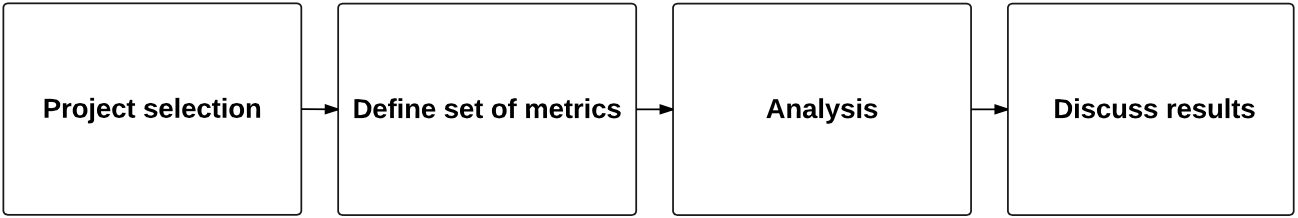
\includegraphics[width=1\textwidth]{figures/approach}
\end{figure*}

The goal of our project is to distinguish Defect Debt from Bugs. In order to do that we conducted a study using one large open source project, Google Chrome. We present our approach overview in \ref{fig:approach}. First, we extract data from the source code and from the issuer tracker repositories. Second,  we process the data to find relevant attributes and link them together. Third, we define our set of metrics and models. Then we analyze our results and answer the research questions. In the following sections we explain in details each one of the steps in our approach.   

\subsection{Data Extraction}

We use Google Chrome to conduct our study. Chrome is a large, mature open source software mostly written in C/C++. The criteria to select this project are its size, the easy access to its source code repository and to the its issuer tracker. Other than that, we had at our disposal some of the desired data that was used in a previous study. This data contained 47.938 html files and 5 tables. Each one of the files represent a bug extracted from the issue tracker. The tables contains the necessary information to link issues files, bugs and commits together. More details about the project can be found in table \ref{tab:project_details}.

To complement the data necessary to our study, we extract from the Chrome Releases website \ref{chrome_releases} the release date of each stable version release, the tag of the release and the release number. Then we store this data in our database.
 
In order to have all the source code available we clone Chromium Git repository. 

\subsection{Process data and find attributes}

After the extraction we process the data and search for attributes that will help us in our analysis. 

First, we create the attributes to store the date that the bug was reported, the release which the bug was reported, the number of comments found in the bug and the release that the bug was commited. Then we process the issues files to get the reported date and the number of comments of each bug. The release and commit dates we get from the release table. 

Second, we create the attributes to store information about the commit classification and the files included in the commit. We use Commit Guru\ref{commit_guru} to gather this information. Commit Guru is an on-line tool, which run a series of source code analysis in a given git repository url. The commit classification is based on the commit message and is used to predict the intend of a change. The process uses key words and expressions that are strong indicators of intend, like `add' or `bug fix'. The possibles classifications are `Feature Addition', `Corrective', `Preventative', `Merge', `Non Functional', `Perfective' and without classification.

Third, we create a table to store metrics values. We collect our metrics using Understand a code analysis tool. This tool can analyze different releases of a project and create a separated database containing several metrics \ref{understand_metrics} for each one of the processed releases. It is possible to access these databases through an API and collect the processed information. We checkout 18 stable releases from our Chrome repository based on the collected tag information from the selected releases. Due to the size of the project and time constraints we use only the `chrome' directory without the third party libraries in our analysis. The whole process took approximately 16 hours and generated more than 2GB of data. 

Different scripts written in Python and SQL were developed during this step in order to make this process automatic and easily reproducible. We provide the link\footnotetext{https://github.com/maldonado/soen6611} to these files just to evaluation purposes. 

\subsection{Link data}

\subsection{Define metrics}


